% =============================================================================
% Turkish Journal of Electrical Engineering & Computer Sciences (elektr class)
% Multiplicative information gating: decomposing news into novelty, materiality,
% and polarity for calibrated selective forecasting.
%
% Every quantitative result is a measured statistic from the authors' deployed
% system or its live append-only ledger; figures are vector (pgfplots/TikZ) and
% can be exported as separate PDFs for submission. Illustrative examples are
% labelled as such and carry no performance claim.
% =============================================================================
\documentclass{elektr}
\usepackage{hyperref}
\hypersetup{
colorlinks=true,
urlcolor=black,
citecolor=blue}
\usepackage[all]{xy,xypic}
\usepackage{amsfonts,amssymb,amsmath,amsgen,amsopn,amsbsy,theorem,graphicx,epsfig}
\usepackage{eufrak,amscd,bezier,latexsym,mathrsfs,eurosym,enumerate}
\usepackage[utf8]{inputenc}
\usepackage[english]{babel}
\usepackage{cleveref,multirow}
\usepackage[dvipsnames]{xcolor}
\usepackage{booktabs}
\usepackage{tikz}
\usepackage{pgfplots}
\pgfplotsset{compat=1.17}
\usetikzlibrary{arrows.meta,positioning,calc,shapes.geometric,fit,backgrounds}
\usepackage[pagewise]{lineno}
\linenumbers

\yil{2026}
\vol{xx}
\fpage{1}
\lpage{12}
\doi{}

\title{Multiplicative information gating: decomposing news into novelty, materiality, and polarity for calibrated selective forecasting}

\author[PARDESHI and DESHMUKH]{
	\textbf{Anandkumar PARDESHI$^{1,*}$\thanks{Correspondence: anand.pardeshi@fcrit.ac.in}~, Sujata DESHMUKH$^{2}$}\\
	$^{1}$Department of Computer Science and Engineering, Fr. C. Rodrigues Institute of Technology,\\ University of Mumbai, Navi Mumbai, India\\
	Anandkumar PARDESHI: \url{https://orcid.org/0000-0002-1825-0097}\\
	$^{2}$Department of Computer Engineering, Fr. C. Rodrigues Institute of Technology,\\ University of Mumbai, Navi Mumbai, India\\
	Sujata DESHMUKH: \url{https://orcid.org/0000-0001-5109-3700}\\[1.8em]
\rec{.. ... 2026}
\acc{.. ... 2026}
\finv{.. ... 2026}
}

\input{elksty.tex}

\setcounter{page}{1}
\begin{document}

\maketitle

\begin{abstract}
Converting a stream of textual events into a trading decision usually reduces each item to a single sentiment polarity and sums, conflating three properties that move prices through different channels: the direction of the news, how surprising it is, and how much it bears on value. We propose multiplicative information gating, in which each event is decomposed into polarity, novelty, and materiality and combined as their product, so that any near-zero factor vetoes the signal. A large language model supplies the three scores from calibration-anchored prompts; the resulting signal feeds a probabilistic forecaster whose output is calibrated and then passed through a conviction gate that may abstain. We prove that the product is the canonical combiner under per-axis multiplicative scaling, with veto and sign acting as consistency conditions, and we bound the signal by its weakest factor. The framework is market-agnostic; we instantiate it on exchange-traded equities using measured numbers only. On a live append-only ledger of 621 resolved forecasts, nominal 90\% price intervals achieved 70.7\% empirical coverage, confirming that deployed uncertainty is not self-correcting. An offline three-stage recalibration that first repaired a stacking domain mismatch cut expected calibration error from 0.35 to 0.05 without changing accuracy. Single-name next-period direction was unpredictable beyond drift (50.1\% out-of-sample, ranking area under the curve near 0.47), so value had to come from selection rather than ordering: a conviction gate that abstains on roughly 94\% of cases raised the realised 30-day hit rate to 60.6\% against a 58.0\% base (95\% interval 58.8 to 62.4), winning in four of five test years. The contribution is a reusable, auditable recipe whose text and decision stages obey one selective principle.
\keywords{Calibration, selective prediction, natural language processing, large language models, financial forecasting, sentiment analysis}
\end{abstract}

% ============================================================================
\section{Introduction}
\label{sec:intro}
% ============================================================================
A growing class of decision systems reads text and acts on it: news headlines, filings, social posts, and support tickets arrive as timestamped streams, and somewhere downstream a model turns them into a number that drives an action. The dominant recipe scores each item for sentiment polarity, averages the scores, and feeds the average to a predictor \cite{tetlock2007,loughran2011}; the financial literature has used it to show that media tone carries return-relevant information \cite{tetlock2007,antweiler2004}. But the recipe rests on an assumption that breaks down on the events that matter most.

Sentiment polarity answers one question: is this good or bad? It is silent on two others that a careful reader weighs instinctively: is the news actually new, or a restatement of something the market priced weeks ago, and does it bear on value, or is it cosmetic? A glowing but stale press release can score the same polarity as a quietly worded regulatory filing that threatens the firm's existence, even though their price impact differs by orders of magnitude. When such items are summed, the loud and empty ones drown out the rare informative ones, because averaging rewards volume over relevance.

We take the position that a textual event has at least three separable properties, each governing price impact through a different channel: \emph{polarity}, the sign of the implied value change; \emph{novelty}, how much genuinely new information the item carries relative to what was already known; and \emph{materiality}, how sensitive fundamental value is to the event, independent of its sign or freshness. Our proposal, multiplicative information gating, keeps the three axes separate and combines them as a product: polarity times novelty times materiality. Because the factors are bounded and at least two are non-negative, the product behaves like a soft logical AND---a stale or immaterial item produces a signal near zero no matter how strong its polarity, so a single weak factor vetoes the whole event. Plain averaging has no such property, which is what lets a multiplicative signal keep a live position from reacting to noise that merely sounds important.

Two practical questions follow. First, who supplies the three scores? Hand-built dictionaries capture polarity passably \cite{loughran2011} but struggle with novelty and materiality, which require world knowledge and context; we use a general-purpose instruction-tuned large language model, prompted with explicit numerical anchors so that its scores are reproducible and comparable across items \cite{brown2020,lopezlira2023}. Second, once the gated signal enters a forecaster, how do we keep the system honest about what it does and does not know? The same gating principle reappears at the decision stage: a forecaster operating near the efficient-market limit \cite{fama1970} is mostly wrong about direction, so what it owes the user is not a confident guess on every name but a calibrated probability and the discipline to abstain when conviction is low \cite{chow1970,elyaniv2010,geifman2017}. Calibration and selective abstention are the decision-stage counterpart of the text-stage veto: each narrows what the system will commit to in return for being dependable on the rest.

We make the argument concrete on equities, where the data are public and the stakes are real, but the construction is market-agnostic and, we argue, domain-agnostic. The contributions are as follows.
\begin{enumerate}
\item We formalise multiplicative information gating: a decomposition of a textual event into polarity, novelty, and materiality, combined as a product, with a relevance-weighted aggregation to the entity level (Section~\ref{sec:method}). We prove a veto bound and show that, under five stated axioms whose substantive content is per-axis multiplicative scaling, the product is the canonical combiner (Section~\ref{sec:theory}).
\item We give a reproducible scoring protocol in which a large language model returns the three axes from calibration-anchored prompts, with a deterministic lexicon fallback and persistent memoisation so that a given item is scored once (Section~\ref{sec:scoring}).
\item We couple the gated text signal to a calibrated, selective forecaster, and we report measured results only: live-ledger interval coverage, a three-stage calibration that repairs a stacking domain mismatch, a verified accuracy ceiling, and a conviction gate evaluated walk-forward over an eight-year span, 2018 to 2026 (Section~\ref{sec:results}).
\end{enumerate}
Throughout, we are deliberate about what we can and cannot claim. The deployed ledger does not record per-event return labels, so we do not assert an isolated alpha for the text decomposition; its contribution is argued from its formal properties and its place in a pipeline whose end-to-end behaviour we do measure. Section~\ref{sec:discussion} returns to this restraint.

% ============================================================================
\section{Related work}
\label{sec:related}
% ============================================================================
\textbf{Text and returns.} The idea that media content carries return-relevant information is well established. Tetlock \cite{tetlock2007} linked pessimistic media tone to downward pressure and subsequent reversal; Antweiler and Frank \cite{antweiler2004} studied message-board activity; Loughran and McDonald \cite{loughran2011} showed that finance-specific dictionaries matter because general-purpose ones mislabel domain terms. Supervised text models tailored to returns improve on dictionaries \cite{ke2019}, and pre-trained language models, including finance-tuned variants, now dominate sentiment extraction \cite{araci2019,huang2023}. Most of this work, however, treats the per-item output as a scalar polarity and aggregates by counting or averaging; the novelty and materiality of an item are handled, if at all, by ad hoc filters rather than as first-class, separately scored quantities. Boudoukh et al.\ \cite{boudoukh2019} is a notable exception in spirit: identifying which news is relevant sharply changes the measured information content. We make relevance and surprise explicit, continuous, and multiplicative. Where Ke et al.\ \cite{ke2019} learn return-predictive word weights by supervising directly on realised returns, we operate in the complementary regime in which no per-item return label is available at scoring time: the three axes are judged zero-shot, and the veto of Section~\ref{sec:theory} guarantees structurally that a stale or immaterial item cannot dominate, however the labels happened to fall.

\textbf{Large language models as scorers.} Instruction-tuned language models can follow rubric-style prompts and emit structured numeric judgements \cite{brown2020}, and finance has adopted them quickly, from domain-specific pre-training at scale \cite{wu2023} to direct tests of whether a general model can read news and anticipate price moves \cite{lopezlira2023}. The self-reported confidence of such models is itself imperfectly calibrated \cite{steyvers2025}, which cautions against reading their raw outputs as probabilities. We do not ask the model to forecast; we ask it to \emph{decompose}, a narrower and more checkable task, constrained by numerical anchors so that two runs on the same item agree. To our knowledge, no prior work scores novelty and materiality as separate, continuous, per-item quantities and makes them multiplicative preconditions for influence with a provable veto: existing pipelines, whether dictionary-based, supervised, or model-driven \cite{loughran2011,ke2019,araci2019,huang2023,lopezlira2023}, reduce the item to one polarity before aggregation.

\textbf{Calibration.} Modern classifiers are often miscalibrated \cite{guo2017}; post-hoc remedies include Platt scaling \cite{platt1999} and isotonic regression \cite{zadrozny2002}, with reliability assessed by expected calibration error and the Brier score \cite{naeini2015,brier1950}. Stacked generalisation \cite{wolpert1992} complicates this: a calibrator fitted on one stage's scores and applied to another silently breaks, a failure we diagnose and repair in Section~\ref{sec:cal}.

\textbf{Selective prediction.} Allowing a model to abstain is an old idea \cite{chow1970} with a modern theory \cite{elyaniv2010,geifman2017} and a distribution-free cousin in conformal prediction \cite{angelopoulos2021,gibbs2021,zaffran2022}. The financial-machine-learning literature, by contrast, is dominated by accuracy and area-under-the-curve reporting, which a long methodological line has shown to be fragile under backtest overfitting and multiple testing \cite{bailey2017,harvey2016}. Deep and ensemble models for markets are now standard \cite{gu2020,kelly2023}, but few report whether their probabilities are trustworthy or whether they know when to stay out; our decision stage is built around exactly those two questions.

% ============================================================================
\section{Materials and methods}
\label{sec:method}
% ============================================================================
\subsection{The multiplicative information model}
\label{sec:model}
Let $e$ denote a textual event (here, a news headline) about an entity (here, a listed equity). We assign $e$ three scores: $s(e)\in[-1,1]$ (polarity), $\nu(e)\in[0,1]$ (novelty), and $\mu(e)\in[0,1]$ (materiality). Polarity is the signed direction of the implied value change; novelty is the degree of genuinely new information, understood as surprise relative to the market's prior; materiality is the sensitivity of fundamental value to the event, regardless of sign. The \emph{event signal} is their product,
\begin{equation}
\label{eq:event}
a(e) \;=\; s(e)\,\nu(e)\,\mu(e)\;\in[-1,1].
\end{equation}
We define the \emph{relevance} of an event as $r(e)=\nu(e)\,\mu(e)\in[0,1]$, so that $a(e)=s(e)\,r(e)$: the event signal is its polarity scaled by how novel-and-material it is. To aggregate the events $\mathcal{E}$ touching one entity into a single signal, we use a relevance-weighted mean restricted to events that clear a materiality floor $\mu_0$,
\begin{equation}
\label{eq:agg}
A \;=\; \frac{\sum_{e\in\mathcal{E}:\,\mu(e)\ge\mu_0} r(e)\,a(e)}{\sum_{e\in\mathcal{E}:\,\mu(e)\ge\mu_0} r(e)}\;=\;\frac{\sum r(e)^2\,s(e)}{\sum r(e)}.
\end{equation}
Relevance enters twice, once inside the event signal and once as the aggregation weight, so an item that is both novel and material dominates quadratically while cosmetic chatter is suppressed. The floor $\mu_0$ discards items below a minimum materiality before weighting; we use $\mu_0=0.15$.

The motivation is a first-order account of price response: if novelty proxies the magnitude of surprise relative to the market's prior and materiality the sensitivity of value to the underlying variable, then to first order the expected value move is the product of a sign, a sensitivity, and a surprise magnitude. Additive sentiment keeps only the sign and discards the coupling, which is why it over-reacts to loud, stale, or immaterial items; \eqref{eq:event} restores the coupling in its simplest form.

\subsection{Why the product, and what it guarantees}
\label{sec:theory}
The multiplicative form is not arbitrary. It is the simplest combiner consistent with how a careful analyst treats the three axes.

\begin{proposition}[Veto bound]
\label{prop:veto}
For every event $e$, $\;|a(e)| \le \min\{\,|s(e)|,\ \nu(e),\ \mu(e)\,\}$. In particular $a(e)=0$ whenever any single factor is zero, and the aggregate satisfies $|A|\le \max_{e}|s(e)|$.
\end{proposition}
\begin{proof}
Each factor lies in $[-1,1]$ with $\nu,\mu\ge 0$, so $|a(e)|=|s(e)|\,\nu(e)\,\mu(e)$ is a product of three numbers of modulus at most one; such a product cannot exceed the modulus of any one of them, which gives the per-event bound and the zero case. For the aggregate, \eqref{eq:agg} gives $A=\big(\sum_e r(e)^2 s(e)\big)/\big(\sum_e r(e)\big)$, so
\[
|A|\;\le\;\frac{\sum_e r(e)^2\,|s(e)|}{\sum_e r(e)}\;\le\;\max_e|s(e)|\;\cdot\;\frac{\sum_e r(e)^2}{\sum_e r(e)}\;\le\;\max_e|s(e)|,
\]
where the last step uses $\sum_e r(e)^2\le\big(\max_e r(e)\big)\sum_e r(e)\le\sum_e r(e)$ because every $r(e)\in[0,1]$. The weights $r(e)^2/\sum_j r(j)$ are non-negative but sub-stochastic, summing to $\sum r^2/\sum r\le 1$; the aggregate is therefore a contraction toward zero of the polarities, never an amplification.
\end{proof}

Proposition~\ref{prop:veto} is the formal content of ``a single weak factor vetoes the event'': a stale ($\nu\!\to\!0$) or immaterial ($\mu\!\to\!0$) item is capped near zero however extreme its polarity. No additive or convex combination of the three axes has this property, because a weighted sum $\alpha s+\beta\nu+\gamma\mu$ is generally nonzero when one term vanishes. We state the design choice as a short characterisation.

\begin{proposition}[Characterisation]
\label{prop:char}
Consider combiners $f(s,\nu,\mu)$ with $s\in[-1,1]$, $\nu,\mu\in[0,1]$ satisfying: (A0) \emph{normalisation}, $f(1,1,1)=1$; (A1) \emph{sign fidelity}, $\operatorname{sign} f=\operatorname{sign} s$; (A2) \emph{veto}, $f=0$ if any of $|s|,\nu,\mu$ is $0$; (A3) \emph{separable monotonicity}, $|f|$ is non-decreasing in each of $\nu$ and $\mu$ for fixed others, and $f$ is non-decreasing in $s$ for fixed $\nu,\mu\ge0$; and (A4) \emph{factor homogeneity}, scaling any single argument by $\lambda\in[0,1]$ scales $f$ by $\lambda$. Then $f(s,\nu,\mu)=s\,\nu\,\mu$.
\end{proposition}
\begin{proof}[Proof sketch]
By (A4) applied to each argument in turn, $f(\lambda_1 s,\lambda_2\nu,\lambda_3\mu)=\lambda_1\lambda_2\lambda_3\, f(s,\nu,\mu)$ for $\lambda_i\in[0,1]$. Writing $s=\operatorname{sign}(s)\,|s|$ and taking $\lambda_1=|s|,\lambda_2=\nu,\lambda_3=\mu$ relative to the unit corner gives $f(s,\nu,\mu)=|s|\,\nu\,\mu\,f(\operatorname{sign}(s),1,1)$. Sign fidelity (A1) forces $f(\pm1,1,1)=\pm c$ with $c=f(1,1,1)$, and the normalisation (A0) fixes $c=1$. Hence $f=s\,\nu\,\mu$; (A2) and (A3) are then automatically satisfied, so they are consistency requirements rather than the active constraints.
\end{proof}

The force of the result lies in homogeneity (A4): it requires each axis to act on its own multiplicative scale, and once that and the normalisation (A0) are granted, the product follows in two lines. The veto and monotonicity conditions (A2, A3) do not by themselves single out the product---many functions satisfy them---so we do not claim the product is the \emph{only} sensible combiner, just the canonical one once per-axis scaling is imposed; and that scaling is exactly the property a position-taking system needs in order to treat freshness and relevance as preconditions for influence rather than as additive contributors.

\subsection{Scoring the three axes with a language model}
\label{sec:scoring}
The decomposition is only as good as the three scores, which we obtain from a general-purpose instruction-tuned large language model (in our deployment, a compact production model, \texttt{Claude Haiku 4.5}), prompted as a quantitative analyst and constrained to return a JSON array of $\{\nu,\mu,s\}$ triples, one per headline, in input order. Two design choices make the scores reproducible.

First, the prompt fixes \emph{numerical anchors} for every axis, so the model maps qualitative judgements onto a shared scale. For novelty, $0.0$ is an exact restatement of news already priced weeks ago, $0.2$ a result that merely met consensus, $0.6$ an unexpected but modest development, and $1.0$ a sudden regulatory ban or fraud disclosure. For materiality, $0.0$ is boilerplate, $0.4$ a contract worth a few percent of revenue, $0.8$ a transformative deal, and $1.0$ an existential event. For polarity, the anchors run from $-1.0$ (fraud allegation, pledge invocation) through $0.0$ (a neutral reshuffle) to $+1.0$ (a large earnings beat with raised guidance). Anchoring narrows the model's effective output distribution and makes two runs on the same item agree closely, which matters because the product in \eqref{eq:event} amplifies disagreement on any one axis.

Second, every scored item is memoised in a content-addressed store keyed by a hash of the entity and the normalised headline, so a given headline is scored once and reused; a run is therefore deterministic given its inputs and cost is bounded. When the model is unavailable, a transparent lexicon fallback assigns polarity from curated bullish and bearish term lists and a conservative fixed novelty and materiality, flagged so that downstream consumers can discount it. The scorer is model-agnostic: any instruction-following model that respects the output contract can be substituted, and the anchors travel with the prompt rather than the weights.

\subsection{From gated signal to calibrated probability}
\label{sec:cal}
The aggregate $A$ of \eqref{eq:agg} is one feature among several entering a hybrid forecaster that blends a gradient-boosted tree ensemble with a recurrent sequence model over price, momentum, trend, reversal, and volatility features to produce, for each name and horizon, a point forecast, a price interval, and a directional probability $\hat p$. We treat the forecaster as a black box; the object of study is not its architecture but its calibration and its willingness to abstain. A probability is only useful if it is calibrated: among names assigned $\hat p\approx0.7$, about $70\%$ should rise. We measure calibration by the expected calibration error over $B$ equal-width bins,
\begin{equation}
\label{eq:ece}
\mathrm{ECE}=\sum_{b=1}^{B}\frac{|G_b|}{N}\,\big|\,\overline{y}_b-\overline{p}_b\,\big|,
\end{equation}
where $\overline{p}_b$ and $\overline{y}_b$ are the mean predicted probability and mean realised outcome in bin $b$, and by the Brier score $\frac1N\sum_i(\hat p_i-y_i)^2$ \cite{brier1950}.

Our first deployed model reported a next-day up-probability near $0.80$ while its realised accuracy sat near $0.51$, an $\mathrm{ECE}$ of $0.345$ and a Brier score worse than a constant $0.5$ forecast. The cause was a stacking domain mismatch \cite{wolpert1992}: an isotonic calibrator had been fitted on the out-of-fold \emph{average of the base learners} but then applied to the \emph{stacked} prediction, a different distribution, and the final blend was never itself calibrated. The repair is a three-stage calibration: (i) refit the isotonic map on the same base-average it was meant to correct, (ii) form the blend, and (iii) fit a final Platt scaler \cite{platt1999} on a held-out fold and apply it to both the test rows and the live row. Equation~\eqref{eq:ece} is the diagnostic at each stage; the effect is reported in Section~\ref{sec:resultcal}.

\subsection{The conviction gate: abstention as decision-stage gating}
\label{sec:gate}
Calibration makes $\hat p$ honest; it does not make it skilful. If short-horizon single-name direction is near-random (Section~\ref{sec:ceiling}), a calibrated probability will sit near the base rate almost everywhere, and acting on every name is pointless. The remedy mirrors the text-stage veto: act only when conviction clears a threshold, and abstain otherwise. For a horizon of $H$ trading days we emit an UP call when the calibrated horizon probability satisfies $\hat p\ge\tau^\star$, and NEUTRAL otherwise. The threshold is chosen on training folds as the smallest $\tau$ whose fired bucket reaches a target precision (here $0.60$) while still firing at least a minimum fraction of the time (here $5\%$):
\begin{equation}
\label{eq:tau}
\tau^\star=\min\Big\{\tau:\ \operatorname{prec}(\tau)\ge 0.60\ \text{and}\ \phi(\tau)\ge 0.05\Big\},
\end{equation}
where $\operatorname{prec}(\tau)=\Pr[y=1\mid \hat p\ge\tau]$ is the fired-bucket precision and $\phi(\tau)=\Pr[\hat p\ge\tau]$ is the firing rate. (We reserve the word \emph{coverage} for interval containment in Section~\ref{sec:resultcov}; the firing rate $\phi$ is its selective-prediction analogue.) The gate is intentionally one-sided: confident DOWN calls on single names are destroyed by the upward drift of equities (Section~\ref{sec:swing}), so the system emits long-or-neutral signals only. Like the event veto, the gate forgoes breadth for dependability, so the quantity worth reporting is precision at a given firing rate rather than accuracy or area under the curve.

Figure~\ref{fig:pipeline} summarises the two gates in one pipeline.

\begin{figure}[t]
\begin{center}
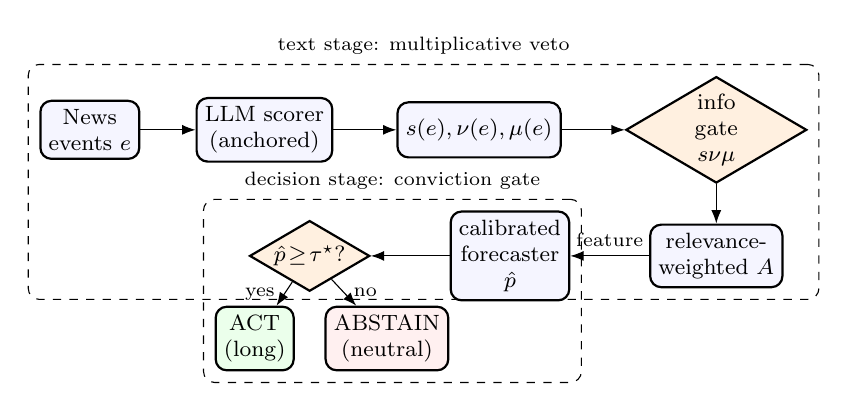
\begin{tikzpicture}[
  font=\footnotesize,
  box/.style={rectangle,rounded corners,draw,thick,align=center,inner sep=3pt,minimum height=7mm,fill=blue!4},
  gate/.style={diamond,draw,thick,align=center,inner sep=1pt,aspect=1.7,fill=orange!12},
  act/.style={rectangle,rounded corners,draw,thick,align=center,inner sep=3pt,fill=green!8},
  ab/.style={rectangle,rounded corners,draw,thick,align=center,inner sep=3pt,fill=red!6},
  >=Latex
]
\node[box] (text) {News\\events $e$};
\node[box,right=7mm of text] (llm) {LLM scorer\\(anchored)};
\node[box,right=8mm of llm] (dec) {$s(e),\nu(e),\mu(e)$};
\node[gate,right=8mm of dec] (g1) {info\\gate\\$s\nu\mu$};
\node[box,below=5mm of g1] (agg) {relevance-\\weighted $A$};
\node[box,left=10mm of agg] (model) {calibrated\\forecaster\\$\hat p$};
\node[gate,left=10mm of model] (g2) {$\hat p\!\ge\!\tau^\star$?};
\node[act,below left=4mm and -2mm of g2] (yes) {ACT\\(long)};
\node[ab,below right=4mm and -2mm of g2] (no) {ABSTAIN\\(neutral)};
\draw[->] (text)--(llm);
\draw[->] (llm)--(dec);
\draw[->] (dec)--(g1);
\draw[->] (g1)--(agg);
\draw[->] (agg)--(model) node[midway,above,font=\scriptsize]{feature};
\draw[->] (model)--(g2);
\draw[->] (g2)-- node[left,font=\scriptsize]{yes} (yes);
\draw[->] (g2)-- node[right,font=\scriptsize]{no} (no);
\begin{scope}[on background layer]
\node[draw,dashed,rounded corners,fit=(text)(g1)(agg),inner sep=4pt,label=above:{\scriptsize text stage: multiplicative veto}] {};
\node[draw,dashed,rounded corners,fit=(model)(g2)(yes)(no),inner sep=4pt,label=above:{\scriptsize decision stage: conviction gate}] {};
\end{scope}
\end{tikzpicture}
\caption{Two gates, one principle. The text stage decomposes each event and vetoes stale or immaterial items through the product $s\nu\mu$; the decision stage calibrates the forecaster's probability and abstains unless conviction clears $\tau^\star$; in both, breadth is given up for dependability. The schematic is conceptual.}
\label{fig:pipeline}
\end{center}\vs{-6mm}
\end{figure}

\subsection{Data, deployment, and evaluation protocol}
\label{sec:data}
The system is deployed on liquid National Stock Exchange of India (NSE) large-capitalisation equities. Two bodies of evidence are used and kept strictly separate. The first is an \emph{offline walk-forward} study on daily data from 2018 to 2026 for a 54-name universe, used to fit and evaluate the forecaster and the gate; all reported offline statistics are out-of-sample under an expanding window, so no future information enters a fitted fold. The second is a \emph{live append-only ledger}: since April 2026 the deployed system has written every issued forecast (entity, timestamp, target date, point forecast, interval, nominal confidence, directional probability, horizon) to a database row that is later stamped with the realised price and outcome. The ledger is first-look only; a forecast is scored against the outcome recorded for its original target date and never retro-edited. It is the strongest evidence we have: produced by the running system, not reconstructed after the fact.

We report three kinds of measured result: interval coverage on the live ledger; the calibration repair and the accuracy ceiling from the offline study; and the selective gate's precision at its firing rate, also offline and walk-forward. No quantity below is illustrative unless its caption says so.

% ============================================================================
\section{Results}
\label{sec:results}
% ============================================================================
\subsection{Deployed uncertainty does not self-correct}
\label{sec:resultcov}
Between 19 April and 12 June 2026 the system issued and later resolved 621 price-interval forecasts on seven NSE large caps (ABB, HDFCBANK, ICICIBANK, INFY, RELIANCE, SBIN, TCS), each carrying a nominal $90\%$ interval with a median half-width of $5.6\%$ of price. Had the intervals been well calibrated, about $90\%$ would contain the realised price; empirical coverage was $70.7\%$ overall, a $19.3$ percentage-point shortfall. The bulk of the forecasts were at the ten-day horizon, where coverage was $69.2\%$ over 575 resolved forecasts; the smaller twenty-day and five-day buckets covered $86.8\%$ and $100\%$ (Table~\ref{tab:cov}, Figure~\ref{fig:results}a). A deployed model's stated confidence was systematically overstated, and nothing in the pipeline noticed on its own: the empirical reason calibration and abstention cannot be afterthoughts.

\begin{table}[h!]
\caption{Live-ledger interval coverage by horizon (NSE large caps, 19 April--12 June 2026). All intervals carry a nominal $90\%$ level.}
\begin{center}
\begin{tabular}{lccc}
\toprule
Horizon & Resolved forecasts & Nominal coverage & Empirical coverage \\
\midrule
5 trading days  & 8   & 90.0\% & 100.0\% \\
10 trading days & 575 & 90.0\% & 69.2\% \\
20 trading days & 38  & 90.0\% & 86.8\% \\
\midrule
All             & 621 & 90.0\% & 70.7\% \\
\bottomrule
\end{tabular}
\label{tab:cov}
\end{center}\vs{-6mm}
\end{table}

\subsection{A stacking domain mismatch, and a three-stage repair}
\label{sec:resultcal}
The offline diagnosis of overconfidence is sharper still; this and the two results that follow are walk-forward measurements, not live-ledger figures. The original next-day directional head reported probabilities clustered near $0.80$ against a realised accuracy of about $0.51$, giving $\mathrm{ECE}=0.345$ and a Brier score above $0.366$, worse than always predicting $0.5$. Tracing the pipeline showed the cause described in Section~\ref{sec:cal}: an isotonic map fitted on the base-learner average was applied to the stacked prediction, and the final blend carried no calibration of its own. The three-stage repair, refitting the isotonic map on its own domain and adding a final Platt scaler on a held-out fold, cut $\mathrm{ECE}$ from $0.345$ to $0.049$ and pulled the reported up-probability back to a realistic neighbourhood of $0.50$. Accuracy did not move: calibration changed what the model \emph{said about its confidence}, not what it predicted. The transferable lesson for any stacked system is that a calibrator is bound to the distribution it was fitted on, and stacking creates more than one such distribution.

\subsection{Single-name direction is unpredictable beyond drift}
\label{sec:ceiling}
Honest calibration exposed an uncomfortable fact that better-looking numbers had hidden. With probabilities pulled back to the base rate, we asked directly whether any robust single-name directional edge survives at short horizons. A cross-sectional model predicting five-day direction across the universe reached $50.09\%$ out-of-fold accuracy, with a ranking area under the curve near $0.49$; that is chance. We confirmed the result five ways, varying the learner and the feature set and gating by trend and market regime; none produced a stable edge over the always-up base rate at the daily scale. This is consistent with the efficient-market prediction for liquid names \cite{fama1970}, and it reframes the problem: if ordering names by predicted return is near-random, ranking-based value is unavailable, and the only lever left is \emph{selection}---the few situations where a calibrated probability departs far enough from the base rate to be worth acting on.

\subsection{Selection recovers a small, stable edge}
\label{sec:swing}
Lengthening the horizon to thirty trading days opens two modest edges: the upward drift of equities (about $58\%$ of thirty-day windows are up) and a small idiosyncratic component captured by a calibrated cross-sectional model on momentum, trend, reversal, and volatility features. Walk-forward from 2018 to 2026 over the 54-name universe (91{,}471 training rows, 50{,}272 out-of-sample rows), the conviction gate of \eqref{eq:tau} settles at $\tau^\star=0.63$. The fired UP bucket achieves $60.6\%$ directional precision against a $58.0\%$ always-up base rate, a net edge of $2.6$ percentage points, while firing on only $5.6\%$ of observations; the model abstains on the remaining $94\%$. The fired bucket pools to $2{,}840$ calls, so the $60.6\%$ precision carries a $95\%$ binomial interval of $58.8$ to $62.4\%$; a one-sided test against the $58.0\%$ base gives $z\approx2.9$ ($p\approx0.002$), so the pooled edge is distinguishable from the base at conventional levels. We do not over-read it: the per-year fired counts are small (Table~\ref{tab:year}), so the year-to-year swings, from $+10.8$ points in 2025 to $-2.4$ in 2024, are within sampling noise, and the honest summary is a small but repeatable tail edge rather than a strong one. The ranking area under the curve is about $0.47$ by construction: the edge lives in the high-conviction tail, not in the ordering, which is what precision at a fixed firing rate registers and area-under-the-curve overlooks. The gate beats its base rate in four of the five test years (Table~\ref{tab:year}, Figure~\ref{fig:results}b); the exception, 2024, appears in the table alongside the rest. Confident DOWN calls, by contrast, reach only about $10\%$ precision out-of-sample, destroyed by drift, which is why the gate never emits them.

\begin{table}[h!]
\caption{Walk-forward selective signal, by test year. Precision is the realised up-rate of the fired high-conviction bucket; base is the always-up rate; fires is the number of high-conviction calls.}
\begin{center}
\begin{tabular}{lcccc}
\toprule
Test year & Fires & Fired-bucket precision & Always-up base & Edge (pp) \\
\midrule
2022 & 365 & 61.6\% & 54.0\% & $+7.6$ \\
2023 & 290 & 68.3\% & 65.3\% & $+3.0$ \\
2024 & 932 & 53.3\% & 55.7\% & $-2.4$ \\
2025 & 822 & 69.0\% & 58.2\% & $+10.8$ \\
2026 & 431 & 54.5\% & 47.1\% & $+7.4$ \\
\midrule
Pooled & 2{,}840 & 60.6\% & 58.0\% & $+2.6$ \\
\bottomrule
\end{tabular}
\label{tab:year}
\end{center}\vs{-6mm}
\end{table}

\begin{figure}[h!]
\begin{center}
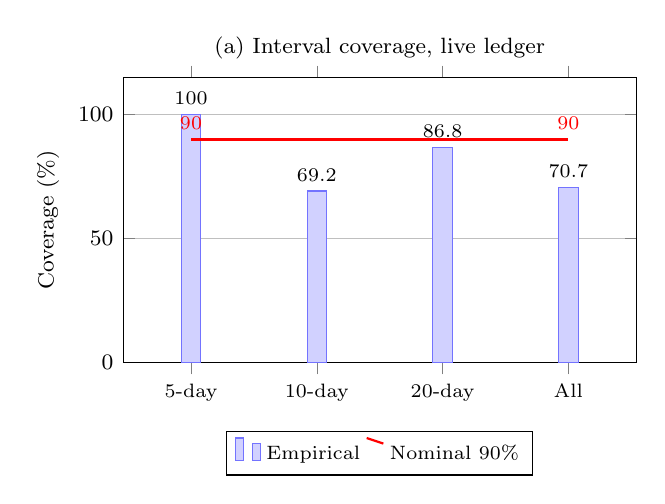
\begin{tikzpicture}
\begin{axis}[
  width=8.1cm, height=5.2cm, font=\footnotesize,
  ybar, bar width=7pt,
  symbolic x coords={5-day,10-day,20-day,All},
  xtick=data, x tick label style={font=\scriptsize},
  ymin=0, ymax=115, ylabel={Coverage (\%)},
  enlarge x limits=0.18, ymajorgrids,
  legend style={at={(0.5,-0.24)},anchor=north,legend columns=2,font=\scriptsize},
  nodes near coords, every node near coord/.append style={font=\scriptsize},
  title={(a) Interval coverage, live ledger}, title style={font=\footnotesize,yshift=-1mm}
]
\addplot[fill=blue!18,draw=blue!55] coordinates {(5-day,100.0)(10-day,69.2)(20-day,86.8)(All,70.7)};
\addplot[sharp plot,thick,red,mark=none,update limits=false] coordinates {(5-day,90)(All,90)};
\legend{Empirical, Nominal 90\%}
\end{axis}
\end{tikzpicture}%
\hfill
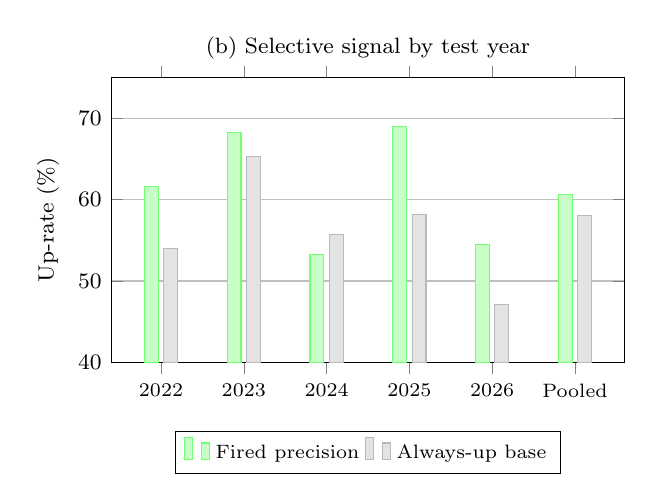
\begin{tikzpicture}
\begin{axis}[
  width=8.1cm, height=5.2cm, font=\footnotesize,
  ybar, bar width=5pt,
  symbolic x coords={2022,2023,2024,2025,2026,Pooled},
  xtick=data, x tick label style={font=\scriptsize},
  ymin=40, ymax=75, ylabel={Up-rate (\%)},
  enlarge x limits=0.12, ymajorgrids,
  legend style={at={(0.5,-0.24)},anchor=north,legend columns=2,font=\scriptsize},
  title={(b) Selective signal by test year}, title style={font=\footnotesize,yshift=-1mm}
]
\addplot[fill=green!22,draw=green!55] coordinates {(2022,61.6)(2023,68.3)(2024,53.3)(2025,69.0)(2026,54.5)(Pooled,60.6)};
\addplot[fill=gray!22,draw=gray!55] coordinates {(2022,54.0)(2023,65.3)(2024,55.7)(2025,58.2)(2026,47.1)(Pooled,58.0)};
\legend{Fired precision, Always-up base}
\end{axis}
\end{tikzpicture}
\caption{Measured behaviour of the two dependability mechanisms. (a) Empirical coverage of nominal $90\%$ intervals on the live ledger by horizon (resolved forecasts: 8, 575, 38, 621 in total). (b) Fired-bucket precision of the conviction gate against the always-up base rate by test year, at about a $5.6\%$ firing rate.}
\label{fig:results}
\end{center}\vs{-6mm}
\end{figure}

\subsection{The veto in action}
\label{sec:vetoaction}
The text stage cannot be evaluated as an isolated alpha, because the deployed ledger does not store per-event return labels; Section~\ref{sec:discussion} weighs this limit. What we can show is that the decomposition behaves as designed. Table~\ref{tab:example} decomposes a small illustrative set of headlines: a glowing but routine in-line result and an emphatic but cosmetic announcement are both gated down, while a quieter disclosure that is genuinely new and material dominates despite its more moderate polarity---the protection Proposition~\ref{prop:veto} guarantees and additive sentiment cannot offer. The example is illustrative of the scoring behaviour and carries no performance claim.

\begin{table}[h!]
\caption{Illustrative decomposition of four headlines for one entity, following the anchors of Section~\ref{sec:scoring}; not a performance measurement.}
\begin{center}
\begin{tabular}{p{6.6cm}cccc}
\toprule
Headline (paraphrased) & Polarity $s$ & Novelty $\nu$ & Material.\ $\mu$ & Signal $a$ \\
\midrule
Quarterly profit in line with consensus, upbeat tone & $+0.30$ & $0.20$ & $0.30$ & $+0.018$ \\
Company reiterates previously announced buyback & $+0.55$ & $0.10$ & $0.40$ & $+0.022$ \\
Unexpected regulator notice on a core product line & $-0.55$ & $0.75$ & $0.80$ & $-0.330$ \\
Routine management reshuffle, no strategic change & $+0.05$ & $0.40$ & $0.15$ & $+0.003$ \\
\bottomrule
\end{tabular}
\label{tab:example}
\end{center}\vs{-6mm}
\end{table}

% ============================================================================
\section{Discussion}
\label{sec:discussion}
% ============================================================================
Every result here turns on the same trade-off. The text-stage veto refuses to let stale or immaterial items contribute, and the decision-stage gate stays out on the great majority of names: the system surrenders any pretence of commenting on everything and earns, in exchange, the right to be believed on the little it does flag. We think this is the correct posture for any model whose outputs are read literally by people with money or safety at stake.

\textbf{Why multiplicative rather than additive.} The veto bound of Proposition~\ref{prop:veto} is not a technicality; it is the whole point. Additive sentiment treats a loud restatement and a quiet revelation as comparable because it scores only tone. The product makes relevance a precondition for influence: we cannot attribute a standalone return to this choice on the present evidence, but the design consequence is testable wherever per-event labels exist---under the product, the events that move the aggregate are those an analyst would flag as new and consequential, and no others.

\textbf{Generality.} Nothing in Section~\ref{sec:method} is specific to equities. Any stream of timestamped textual events that drives a decision has the same three axes: a direction of implied effect, a degree of surprise, and a degree of consequence. Triage of clinical alerts, prioritisation of security or operations tickets, and moderation queues suffer the same failure when collapsed to a single urgency or sentiment score, and could use the same veto against what is loud yet stale or forceful yet immaterial. The decision-stage discipline is equally portable: calibrate, then abstain below a conviction threshold tuned for precision at a chosen firing rate. We chose finance because its outcomes are public and unforgiving, and framed the study as a market-agnostic case so as not to lean on results peculiar to a single venue.

\textbf{Threats to validity and honest limits.} Four limits deserve emphasis. First, the language-model scores are judgements, not measurements: anchoring tightens them but does not make novelty and materiality objective, and a different model or a drifting prompt could shift the scale; the deterministic fallback and the memoisation bound this variance without eliminating it. Second, the live ledger is young, two months and seven names, so its coverage shortfall, though large and consistent at the dominant horizon, is a snapshot rather than a stationary law. Third, and weightiest, we do not have per-event return labels in deployment, so the marginal value of the decomposition over plain polarity is argued from its formal properties and its place in the measured pipeline rather than from an isolated backtest; we would rather say this plainly than manufacture a clean number from a reconstruction, the sort of exercise that invites the backtest-overfitting critique \cite{bailey2017,harvey2016} we take seriously. Fourth, the directional-probability sample on the live ledger is still small, 28 resolved next-period calls, which is why our live claim rests on the 621-forecast interval-coverage evidence and not on a live reliability diagram.

\textbf{Relation to selective and conformal prediction.} The decision gate is an instance of selective classification \cite{chow1970,geifman2017}; what is new is pairing it with a probability whose calibration was itself repaired, and reading both stages as one gating principle. Distribution-free interval methods \cite{angelopoulos2021,gibbs2021,zaffran2022}, adaptive conformal inference in particular, are built for exactly the non-stationary coverage failure of Section~\ref{sec:resultcov}; integrating them is future work.

% ============================================================================
\section{Conclusion}
\label{sec:conclusion}
% ============================================================================
Turning text into decisions should not begin by collapsing every event to a single sentiment number. A textual event carries direction, surprise, and consequence, and these need not move together; taking their product instead of their sum builds a signal in which the weakest axis caps the rest, the safeguard that keeps a live decision from chasing loud noise. We proved that the product is the canonical combiner once per-axis multiplicative scaling is imposed, and bounded the aggregate by its strongest polarity. The same gating logic belongs at the decision stage: on a live deployment ledger, nominal $90\%$ intervals covered only $70.7\%$ of outcomes, so a forecaster has to be calibrated and willing to abstain. An offline three-stage recalibration that first repaired a stacking domain mismatch cut expected calibration error from $0.35$ to $0.05$ without touching accuracy; the corrected probabilities then exposed that short-horizon single-name direction is unpredictable beyond drift; and a conviction gate that stays out on about $94\%$ of names raised the thirty-day hit rate to $60.6\%$ against a $58.0\%$ base, in four of five test years. What ties the two stages together is one rule: give up breadth where the signal cannot be trusted, and commit only where it can. Per-event labelled evaluation of the decomposition and adaptive conformal intervals for the price forecasts are the clear next steps.

% ----------------------------------------------------------------------------
\section*{Acknowledgment and disclaimers}
The authors thank the Department of Computer Engineering, Fr.\ C.\ Rodrigues Institute of Technology, for computing support. The contribution information and the list of authors provided in the manuscript are consistent with the details entered into the CRediT taxonomy. The authors declare that they have no conflict of interest.

\section*{Declaration of generative AI and AI-assisted technologies}
This study uses a large language model as a measurement instrument: an instruction-tuned model (Claude Haiku 4.5, Anthropic) scores news headlines for novelty, materiality, and polarity from the anchored prompt of Section~\ref{sec:scoring}; this use is part of the system under study, and all such outputs were validated against the deterministic fallback and persisted for audit. Separately, during manuscript preparation the authors used a large language model solely to improve the language and readability of author-written drafts; no generative tool produced data, results, figures, or interpretations. The authors reviewed and edited all content and take full responsibility for the publication.

\section*{Data availability statement}
The live forecast ledger and the offline walk-forward statistics underlying Tables~\ref{tab:cov}--\ref{tab:year} and Figure~\ref{fig:results} can be made available by the corresponding author on reasonable request, subject to the platform's terms. Source price data are from public NSE end-of-day records.

% ----------------------------------------------------------------------------
\begin{thebibliography}{99}
\bibitem{tetlock2007} Tetlock PC. Giving content to investor sentiment: the role of media in the stock market. The Journal of Finance 2007; 62 (3): 1139-1168. doi: 10.1111/j.1540-6261.2007.01232.x
\bibitem{loughran2011} Loughran T, McDonald B. When is a liability not a liability? Textual analysis, dictionaries, and 10-Ks. The Journal of Finance 2011; 66 (1): 35-65. doi: 10.1111/j.1540-6261.2010.01625.x
\bibitem{antweiler2004} Antweiler W, Frank MZ. Is all that talk just noise? The information content of internet stock message boards. The Journal of Finance 2004; 59 (3): 1259-1294. doi: 10.1111/j.1540-6261.2004.00662.x
\bibitem{brown2020} Brown TB, Mann B, Ryder N, Subbiah M, Kaplan J et al. Language models are few-shot learners. In: Advances in Neural Information Processing Systems 33 (NeurIPS 2020); Vancouver, Canada; 2020. pp. 1877-1901.
\bibitem{lopezlira2023} Lopez-Lira A, Tang Y. Can ChatGPT forecast stock price movements? Return predictability and large language models. arXiv preprint arXiv:2304.07619, 2023. doi: 10.48550/arXiv.2304.07619
\bibitem{fama1970} Fama EF. Efficient capital markets: a review of theory and empirical work. The Journal of Finance 1970; 25 (2): 383-417. doi: 10.2307/2325486
\bibitem{chow1970} Chow CK. On optimum recognition error and reject tradeoff. IEEE Transactions on Information Theory 1970; 16 (1): 41-46. doi: 10.1109/TIT.1970.1054406
\bibitem{elyaniv2010} El-Yaniv R, Wiener Y. On the foundations of noise-free selective classification. Journal of Machine Learning Research 2010; 11: 1605-1641.
\bibitem{geifman2017} Geifman Y, El-Yaniv R. Selective classification for deep neural networks. In: Advances in Neural Information Processing Systems 30 (NeurIPS 2017); Long Beach, CA, USA; 2017. pp. 4878-4887.
\bibitem{ke2019} Ke ZT, Kelly BT, Xiu D. Predicting returns with text data. National Bureau of Economic Research Working Paper 26186, Cambridge, MA, USA, 2019. doi: 10.3386/w26186
\bibitem{araci2019} Araci D. FinBERT: financial sentiment analysis with pre-trained language models. arXiv preprint arXiv:1908.10063, 2019. doi: 10.48550/arXiv.1908.10063
\bibitem{huang2023} Huang AH, Wang H, Yang Y. FinBERT: a large language model for extracting information from financial text. Contemporary Accounting Research 2023; 40 (2): 806-841. doi: 10.1111/1911-3846.12832
\bibitem{boudoukh2019} Boudoukh J, Feldman R, Kogan S, Richardson M. Information, trading, and volatility: evidence from firm-specific news. The Review of Financial Studies 2019; 32 (3): 992-1033. doi: 10.1093/rfs/hhy083
\bibitem{wu2023} Wu S, Irsoy O, Lu S, Dabravolski V, Dredze M et al. BloombergGPT: a large language model for finance. arXiv preprint arXiv:2303.17564, 2023. doi: 10.48550/arXiv.2303.17564
\bibitem{steyvers2025} Steyvers M, Tejeda H, Kumar A, Belem C, Karny S et al. What large language models know and what people think they know. Nature Machine Intelligence 2025; 7 (2): 221-231. doi: 10.1038/s42256-024-00976-7
\bibitem{guo2017} Guo C, Pleiss G, Sun Y, Weinberger KQ. On calibration of modern neural networks. In: Proceedings of the 34th International Conference on Machine Learning; Sydney, Australia; 2017. pp. 1321-1330.
\bibitem{platt1999} Platt JC. Probabilistic outputs for support vector machines and comparisons to regularized likelihood methods. In: Smola AJ, Bartlett P, Sch\"{o}lkopf B, Schuurmans D (editors). Advances in Large Margin Classifiers. Cambridge, MA, USA: MIT Press, 1999, pp. 61-74.
\bibitem{zadrozny2002} Zadrozny B, Elkan C. Transforming classifier scores into accurate multiclass probability estimates. In: Proceedings of the 8th ACM SIGKDD International Conference on Knowledge Discovery and Data Mining; Edmonton, Canada; 2002. pp. 694-699. doi: 10.1145/775047.775151
\bibitem{naeini2015} Naeini MP, Cooper GF, Hauskrecht M. Obtaining well calibrated probabilities using Bayesian binning. In: Proceedings of the 29th AAAI Conference on Artificial Intelligence; Austin, TX, USA; 2015. pp. 2901-2907.
\bibitem{brier1950} Brier GW. Verification of forecasts expressed in terms of probability. Monthly Weather Review 1950; 78 (1): 1-3. doi: 10.1175/1520-0493(1950)078<0001:VOFEIT>2.0.CO;2
\bibitem{wolpert1992} Wolpert DH. Stacked generalization. Neural Networks 1992; 5 (2): 241-259. doi: 10.1016/S0893-6080(05)80023-1
\bibitem{angelopoulos2021} Angelopoulos AN, Bates S. A gentle introduction to conformal prediction and distribution-free uncertainty quantification. arXiv preprint arXiv:2107.07511, 2021. doi: 10.48550/arXiv.2107.07511
\bibitem{gibbs2021} Gibbs I, Cand\`{e}s E. Adaptive conformal inference under distribution shift. In: Advances in Neural Information Processing Systems 34 (NeurIPS 2021); 2021. pp. 1660-1672.
\bibitem{zaffran2022} Zaffran M, F\'eron O, Goude Y, Josse J, Dieuleveut A. Adaptive conformal predictions for time series. In: Proceedings of the 39th International Conference on Machine Learning; Baltimore, MD, USA; 2022. pp. 25834-25866.
\bibitem{bailey2017} Bailey DH, Borwein J, Lopez de Prado M, Zhu QJ. The probability of backtest overfitting. Journal of Computational Finance 2017; 20 (4): 39-69. doi: 10.21314/JCF.2016.322
\bibitem{harvey2016} Harvey CR, Liu Y, Zhu H. $\ldots$ and the cross-section of expected returns. The Review of Financial Studies 2016; 29 (1): 5-68. doi: 10.1093/rfs/hhv059
\bibitem{gu2020} Gu S, Kelly B, Xiu D. Empirical asset pricing via machine learning. The Review of Financial Studies 2020; 33 (5): 2223-2273. doi: 10.1093/rfs/hhaa009
\bibitem{kelly2023} Kelly BT, Xiu D. Financial machine learning. Foundations and Trends in Finance 2023; 13 (3-4): 205-363. doi: 10.1561/0500000064
\end{thebibliography}

\end{document}
